\chapter*{Введение}                         % Заголовок
\addcontentsline{toc}{chapter}{Введение}    % Добавляем его в оглавление

Гидроразрыв пласта (ГРП) — один из эффективных методов интенсификации нефтеотдачи. Суть данного метода заключается в следующем. При помощи закачки вязкой жидкости на забое скважины создается избыточное давление, достаточное чтобы преодолеть горные напряжения и разорвать горную породу. Порода разрывается вдоль поверхностей минимальных напряжений в пласте, и за счет гидродинамического воздействия жидкости в породе начинает расти и раскрываться трещина. Ввиду сложности физических процессов и недоступности прямому наблюдению развития трещины гидроразрыва пласта, для оценки технологических параметров при проведении ГРП и геометрических размеров созданной трещины применяют специализированное программное обеспечение — симуляторы гидроразрыва пласта.

Для коммерческих симуляторов гидроразрыва помимо точности численных методов для моделирования ГРП не менее важна скорость расчётов. Применяемые в научной практике симуляторы ГРП, основанные на методе конечных элементов (МКЭ), позволяют решать задачи для неоднородной среды и учитывать факторы неоднородного распределения порового давления и температуры, однако требуют больших вычислительных ресурсов. Для коммерческого применения или для проведения оптимизационных расчетов применяются менее ресурсоемкие подходы, основанные на упрощающих предположениях о свойствах описываемой среды.

\begin{figure}[htbp]
    \centering
    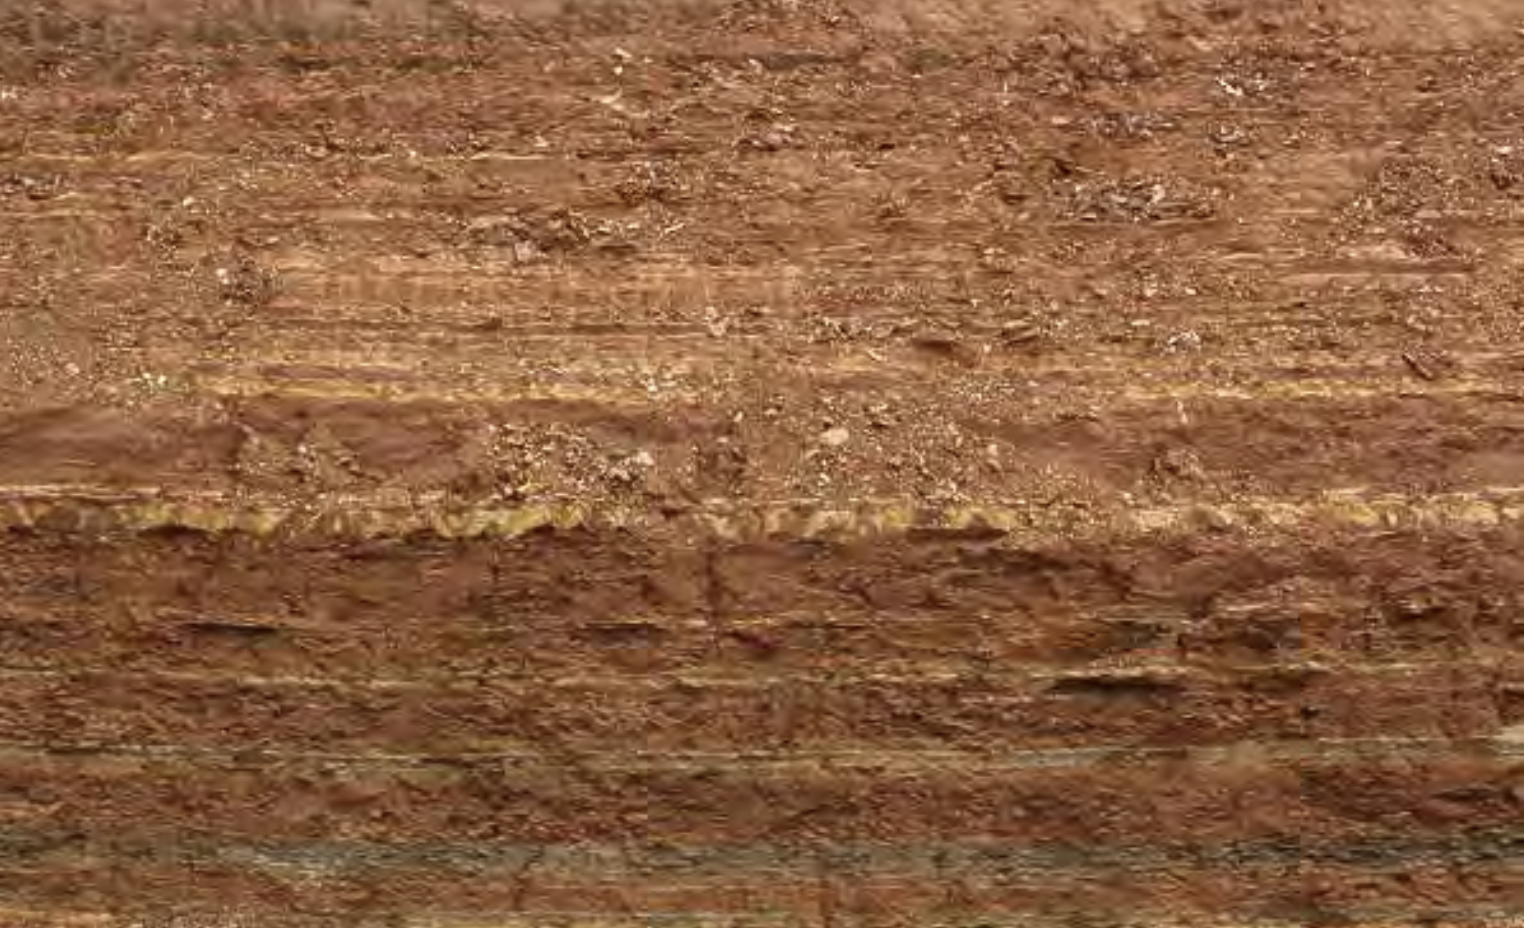
\includegraphics[width=0.8\textwidth]{layered-structure.png}
    \caption{Слоистая структура горной породы.}
\end{figure}

Обычно для математического моделирования ГРП целевой пласт представляется в виде слоистой среды, где каждый слой считается упругим изотропным сплошным телом, обладающим своими модулями упругости. Одной из используемых в практике является модель Planar3d ILSA \cite{DONTSOV201753}, используется для моделирования плоских магистральных трещин ГРП. Она основана на вариации метода граничных элементов --- методе разрывных смещений (МРС), \cite{dispalecement_discontinuty_Crouch1983}), в котором расчетная сетка строится только в плоскости трещины. Это позволяет уменьшить размерность матрицы упругости на единицу за счет сведения пространственной задачи к уравнениям на границе области с использованием аналитического решения уравнений упругости для однородной изотропной среды \cite{Peir2008}. Для слоистой среды не существует аналитического выражения для коэффициентов матрицы упругости, поэтому для обобщения данного метода использует следующие подходы.

Первый заключается в гомогенезации (осреднении) модулей упругости по всем слоям \cite{DONTSOV2021108144}. Преимуществом данного подхода является относительно простая реализация, за счет введения средних модулей упругости и сведения задачи к однородной изотропной среде. Однако данный подход не применим для слоистых структур с большой разницей упругих модулей и сред с включением тонких жестких пропластков.

Второй подход основан на численном построение матрицы упругости \cite{Siebrits_Peirce_2002,Peirce2001TheSF,Peirce2001UniformAA,Linkov1992}. Для этого применяют двумерное преобразование Фурье для определяющих уравнений упругой среды и далее, учитывая условия непрерывности компонент вектора смещений и нормальной нагрузки на границе раздела слоев, решают связанную задачу. После этого матрицу упругости восстанавливается путем применения обратного дискретного преобразования Фурье к полученному решению.

Целью данной работы является реализация метода построения численной матрицы упругости для слоистой среды с неоднородностью по модулям упругости и внедрение его в модель Planar3d ILSA, реализованной ранее в лаборатории цифровых и интеллектуальных систем добычи углеводородов в Институте гидродинамики им. М. А. Лаврентьева СО РАН. В работе проведен параметрический анализ задачи и показано существенное влияние неоднородности модулей упругости на геометрию трещины ГРП. Проведено сравнение влияния неоднородности сжимающих напряжений и модулей упругости слоев на геометрию финальной трещины ГРП. Изучено влияние тонких жестких пропластков на раскрытие трещины, что важно при расчете переноса расклинивающего агента (проппанта) и других компонент жидкости по трещине.


\clearpage